\documentclass{beamer}
\newcommand{\myfont}{\rmfamily\normalsize\upshape\mdseries}
\newcommand{\degree}{^\circ}
\newcommand{\R}{\mathbb{R}}
\newcommand{\F}{\mathbb{F}}
\title{\sffamily Review VIII}
\subtitle{\textbf{Integral}\\ }
\institute[UM-SJTU JI]{University of Michigan-Shanghai Jiao Tong University Joint Institute}
\author{Kulu}
\usepackage{graphicx}
\usepackage{picinpar}
\usepackage{indentfirst}
\usepackage{chemformula}
\usepackage{geometry}
\usepackage{subfigure}
\usepackage{appendix}
\usepackage{amsfonts,amsmath,amssymb}
\usepackage{enumerate}
\usepackage{float}
\usepackage{geometry}
\usepackage{latexsym}
\usepackage{listings}
\usepackage{multicol,multirow,multido}
\usepackage{tabularx}
\usepackage{ulem}
\usepackage{tikz}
\usepackage{xcolor}
\usepackage{cite}
\usepackage{setspace}
\usepackage{textpos}
\usepackage{booktabs}
\usepackage{mathtools, nccmath}
\usepackage{hyperref}
\usetheme[dove]{Boadilla}
\usecolortheme{dolphin}
\useoutertheme{miniframes}

\begin{document}
\usebackgroundtemplate{\tikz\node[opacity=0.05]{
        \centerline{
\includegraphics[
                height=\paperheight]{kulu.jpg}}
    };}
\begin{titlepage}
    \begin{center}
        VV186 - Honors Mathmatics II
    \end{center}
\end{titlepage}
\myfont

\begin{frame}
    \begin{figure}[htbp]
        \centering
        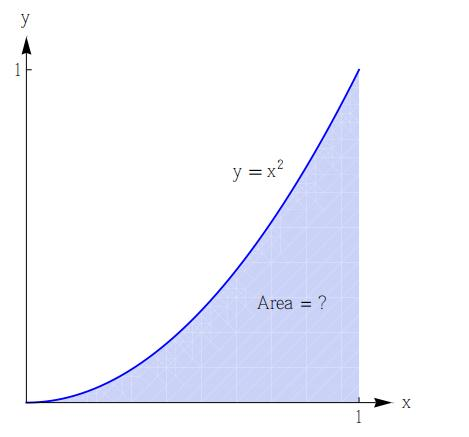
\includegraphics[width=8cm]{pic1.png}
    \end{figure}
\end{frame}

\begin{frame}
    \begin{figure}[htbp]
        \centering
        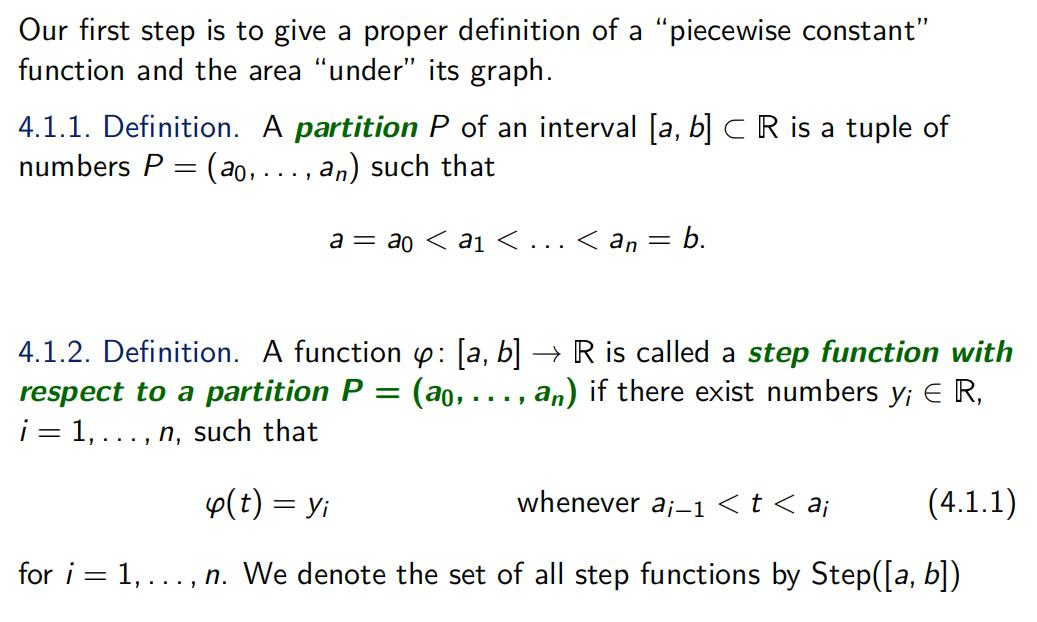
\includegraphics[width=12cm]{pic2.png}
    \end{figure}
\end{frame}

\begin{frame}
    \begin{figure}[htbp]
        \centering
        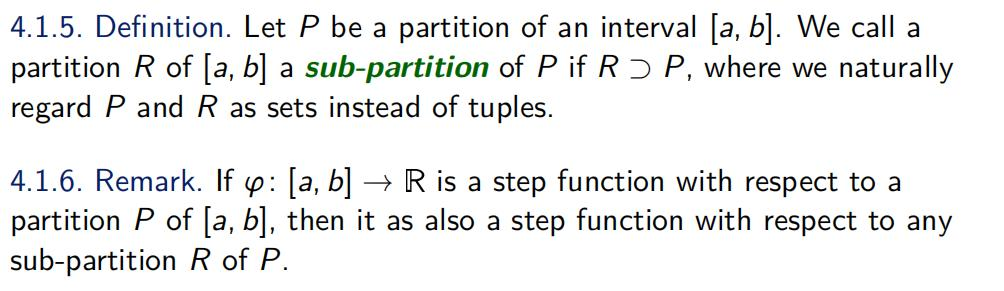
\includegraphics[width=12cm]{pic3.png}
    \end{figure}
    \begin{figure}[htbp]
        \centering
        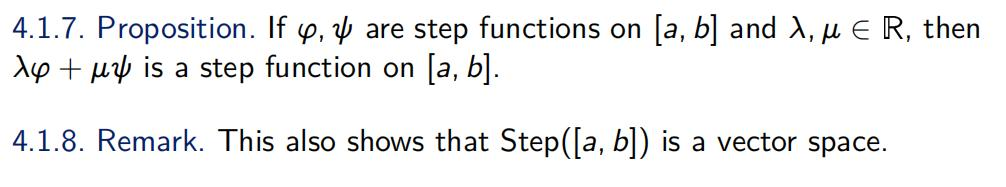
\includegraphics[width=12cm]{pic4.png}
    \end{figure}
\end{frame}

\begin{frame}
    \begin{figure}[htbp]
        \centering
        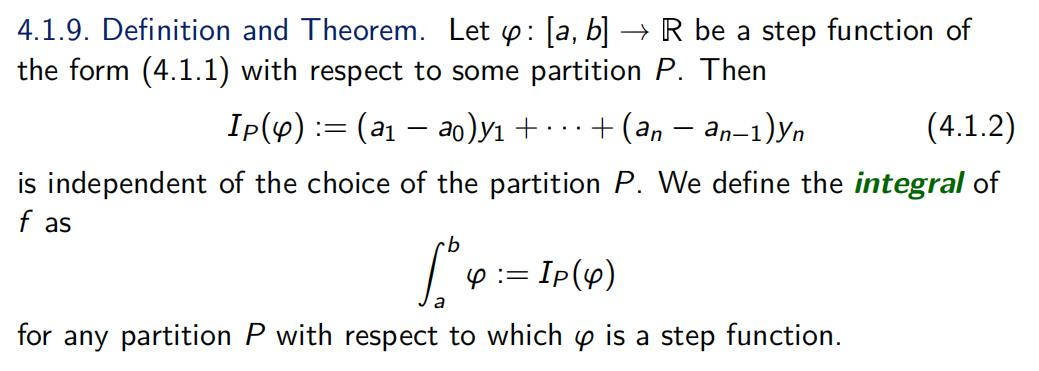
\includegraphics[width=12cm]{pic5.png}
    \end{figure}

    \begin{figure}[htbp]
        \centering
        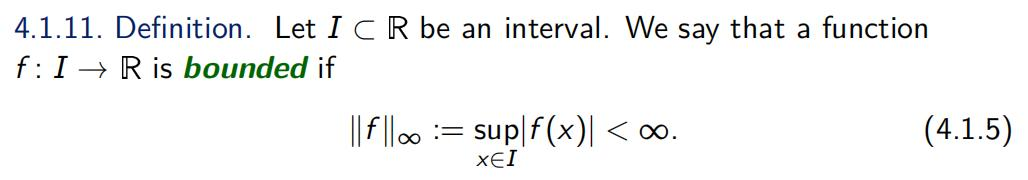
\includegraphics[width=12cm]{pic6.png}
    \end{figure}
\end{frame}

\begin{frame}
    \begin{figure}[htbp]
        \centering
        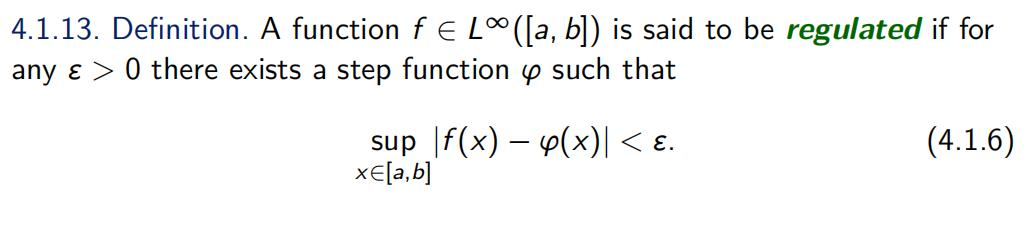
\includegraphics[width=12cm]{pic7.png}
    \end{figure}
    \begin{figure}[htbp]
        \centering
        
\includegraphics[width=12cm]{pic8.png}
    \end{figure}
    \begin{figure}[htbp]
        \centering
        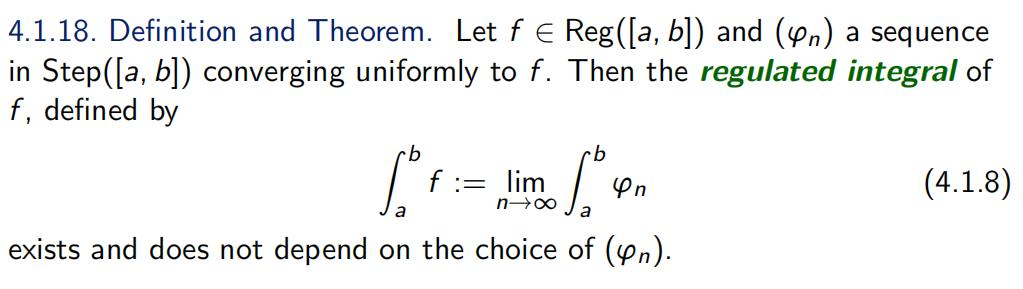
\includegraphics[width=12cm]{pic9.png}
    \end{figure}
\end{frame}

\begin{frame}
    \begin{figure}[htbp]
        \centering
        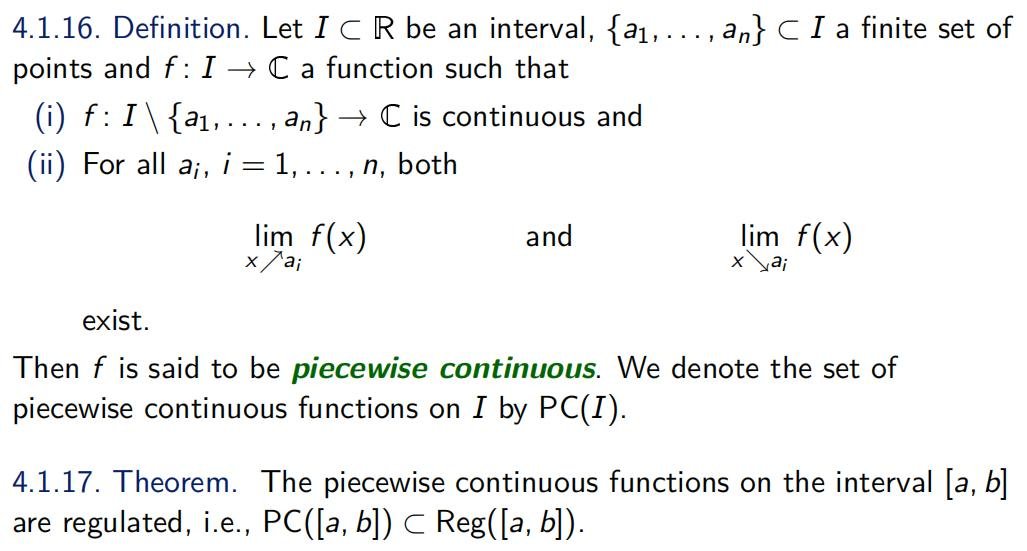
\includegraphics[width=12cm]{pic10.png}
    \end{figure}
\end{frame}

\begin{frame}
    \begin{figure}[htbp]
        \centering
        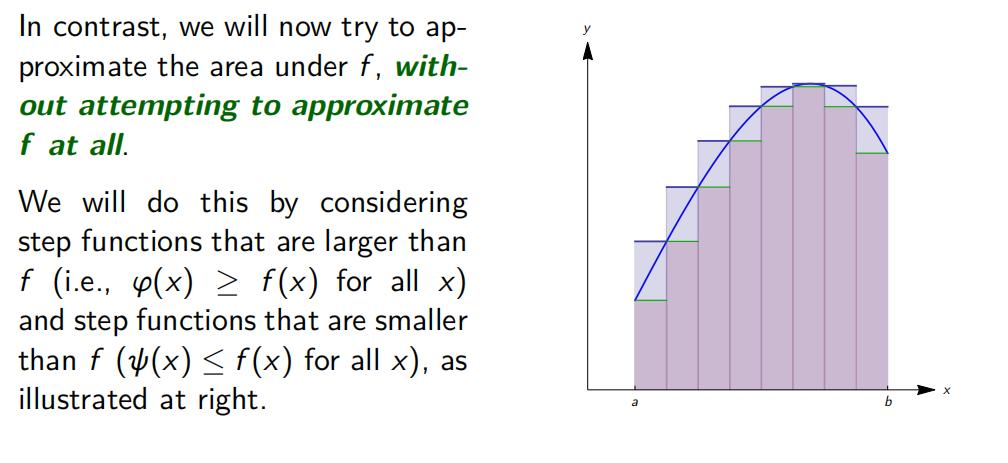
\includegraphics[width=12cm]{pic11.png}
    \end{figure}
\end{frame}

\begin{frame}
    \begin{figure}[htbp]
        \centering
        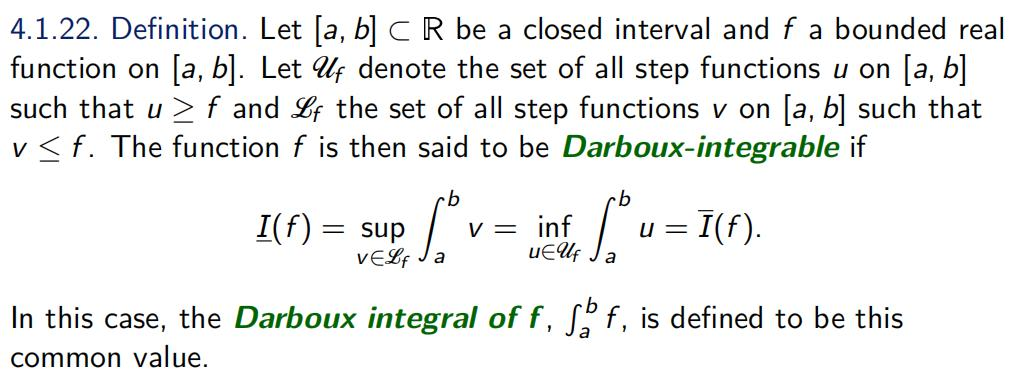
\includegraphics[width=12cm]{pic12.png}
    \end{figure}
\end{frame}

\begin{frame}
    \begin{figure}[htbp]
        \centering
        
\includegraphics[width=12cm]{pic13.png}
    \end{figure}
    \begin{figure}[htbp]
        \centering
        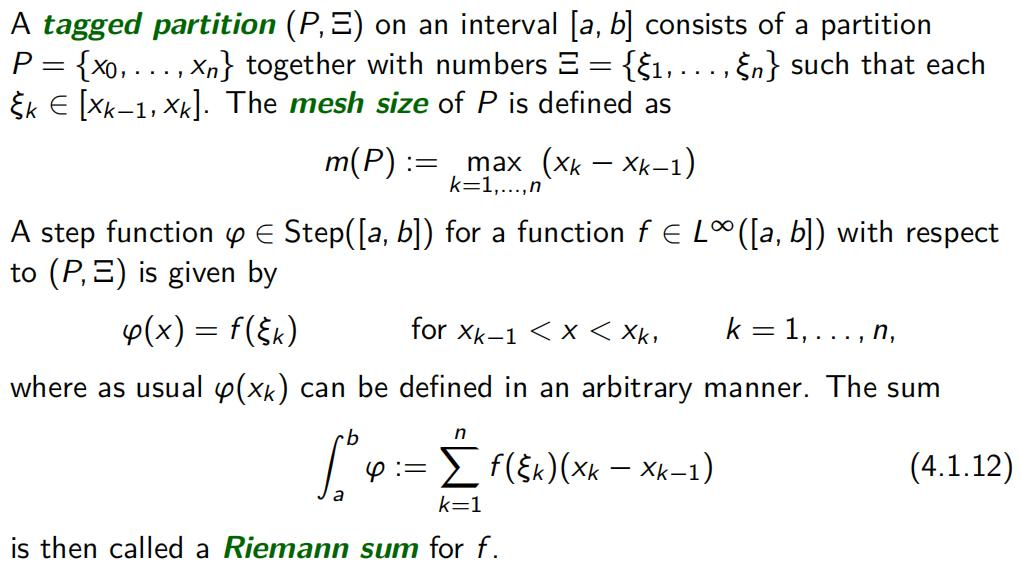
\includegraphics[width=12cm]{pic14.png}
    \end{figure}
\end{frame}

\begin{frame}
    \begin{figure}[htbp]
        \centering
        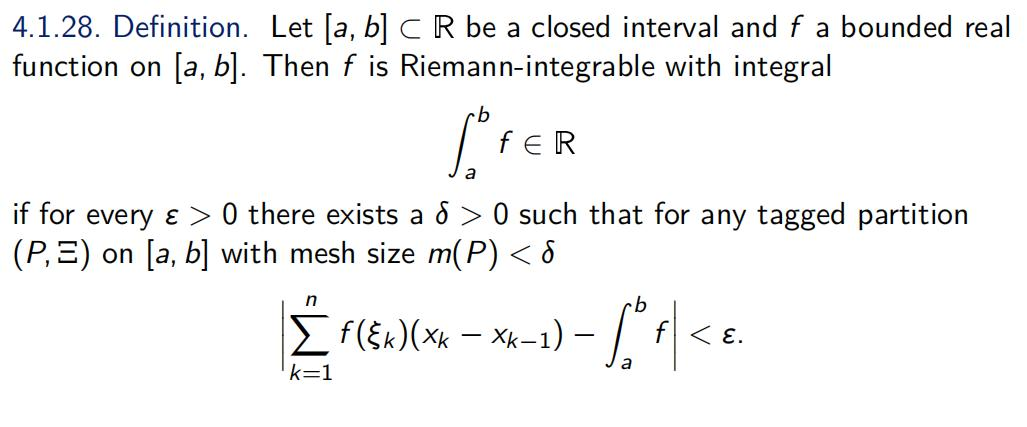
\includegraphics[width=12cm]{pic15.png}
    \end{figure}
    \begin{figure}[htbp]
        \centering
        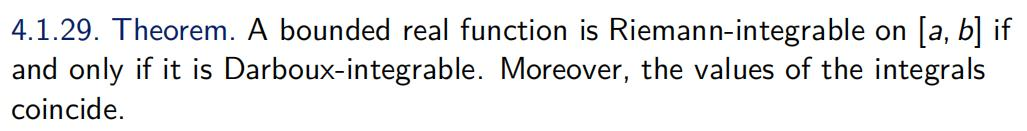
\includegraphics[width=12cm]{pic16.png}
    \end{figure}
\end{frame}


\begin{frame}
    \frametitle{Integration Method}
    Method0: Symmetry\\
    \vspace{1em}\hspace{1em}
    Suppose $f~(x)$ is an odd integrable function, then $$\int_{-a}^a f~(x)dx=0$$
    \\
    \vspace{1em}
    \hspace{1em} Exercises: For $a>0$, calculate
    $$\int_{-a}^a \frac{\cos(x)}{1+even(x)^{odd(x)}} dx$$
    where $even(x)$ is a continuous strictly positive even function, and $odd(x)$ is an odd function
\end{frame}
\begin{frame}
    \frametitle{Integration Method}
    Method1: Recite!\\
    \vspace{1em}
    Common indefinite integrals include:
    \begin{itemize}
        \item $\int x^\alpha dx=\frac{x^{\alpha+1}}{\alpha+1} +C$
        \item $\int e^x dx=e^x +C $
        \item $\int \frac{1}{x}dx=\ln(|x|)+C$
        \item $\int \cos x~ dx = \sin x +C$
        \item $\int \sin x~ dx = -\cos x +C$
        \item $\int \frac{1}{1+x^2} dx = arctan(x) +C$
        \item $\int \ln(x)= ?$
    \end{itemize}
    For more complex integrals, we need other theorems to help us evaluate
    them.
\end{frame}
\begin{frame}
    \frametitle{Exercise}
    Calculte the following integrals:
    \begin{itemize}
        \item $$\int \frac{2}{\sqrt{x^3}} dx$$
        \item $$\int \frac{1}{x^2+6x+5} dx$$
    \end{itemize}
    \vspace{1em}
    \hspace{1em}
    \itshape
    Comment. Partial fraction is sometimes powerful!\myfont
\end{frame}
\begin{frame}
    \frametitle{Integration Method}
    Method2: Substitution!\\
    \vspace{1em}
    \begin{itemize}
        \item Let $u=g(x)$.
        \item Compute $du=g'(x)$.
        \item Substitute $g(x)=u$ and $g'(x)=du$. \textbf{At this moment, only $u$, no $x$ !!!}
        \item Calculate the above integral of $u$, it should be easier.
        \item Replace $u$ by $g(x)$ to get the result with $x$.
        \item For definite integral, pay attention to the range.
    \end{itemize}
    \begin{block}{Demo}
        $$\int sin(x) cos(x) dx$$
    \end{block}
\end{frame}
\begin{frame}
    \frametitle{Exercise}
    Calculte the following integrals:
    \begin{itemize}
        \item $$\int_{-1}^3 \sqrt{9-x^2} dx$$
        \item $$\int \tan(x) dx$$
        \item $$\int \frac{x}{3x^2+6x+10} dx$$
        \item $$\int \frac{e^{4x}}{1+e^{2x}} dx$$
    \end{itemize}
\end{frame}
\begin{frame}
    \frametitle{Integral Method}
    Method3: Integration by part!\\
    \vspace{1em}

    For definite integral:
    $$\int_a^b f~'(x)g(x) dx=f~(x)g(x) \Big|_a^b-\int_a^b f~(x)g'(x) dx$$
    For indefinite integral:
    $$\int f~'(x)g(x) dx=f~(x)g(x) -\int f~(x)g'(x) dx$$
    Demo:
    $$\int x \sin (x) dx$$
\end{frame}
\begin{frame}
    \frametitle{Exercise}

    \begin{itemize}
        \item $$\int x^2 e^{-x} dx$$
        \item $$\int (\ln x)^2 dx$$
        \item $$\int_0^{\frac{\pi}{2}} \sin^n x ~dx$$
    \end{itemize}

\end{frame}

\begin{frame}
    \frametitle{Reference}
    \begin{itemize}
        \item 2021-Vv186 TA-Niyinchen
    \end{itemize}
\end{frame}
\begin{frame}
    \frametitle{End}
    \centering
    \LARGE{Thanks!}


\end{frame}
\end{document}